\documentclass[12pt, letterpaper]{article}
\usepackage{graphicx}

\title{Visualizing ocean data with OceanSpy}
\author{Sourav Barua}
\date{August 5, 2020}

\begin{document}

\maketitle

\section{Introduction}
Ocean Current Simulation using numerical circulation models have become so realistic at present. These simulation models generate a large volume of model output data, making the analysis of model data harder. Using OceanSpy, model data can be easily analyzed in the way observational oceanographers analyze field measurements.  OceanSpy\footnote{https://github.com/hainegroup/oceanspy} is an open-source and user-friendly Python package that enables scientists and interested amateurs to analyze and visualize ocean model datasets.

In this project, I use the demo data provided by OceanSpy to demonstrate their two plotting method TS\_diagram() and horizontal\_section() to create a Temperature vs. Salinity plot and a temperature with depth plot. 
 


\section{Methods}

\subsection{Dataset}
The dataset used for this demonstration is the demo date provided by OceanSpy. These data contain High-resolution (~2km) numerical simulation covering the east Greenland shelf (EGshelf), and the Iceland and Irminger Seas (IIseas) forced by the Arctic System Reanalysis (ASR). These data can be downloaded from https://livejohnshopkins-my.sharepoint.com/:u:/g/personal/
malmans2\_jh\_edu/EXjiMbANEHBZhy62oUDjzT4BtoJSW2W0tYtS2qO8\_SM5m
Q?download=1



\section{OceanSpy for Ocean data visualization}

OceanSpy provides different plotting functionalities that makes the process of plotting of different oceanographic data easy and efficient. OceanSpy builds on software packages developed by the Pangeo community, in particular xarray, dask, and xgcm. 

\subsection{TS\_diagram() method}
The TS\_diagram method inside the oceanspy.plot module plots temperature-salinity plots of the OceanDataset object. I created a GenerateTvsSalinityPlot.py file that downloads the example data file provided by OceanSpy and then uses the method TS\_diagram() to draw a Temperature vs salinity graph.  

\subsection{horizontal\_section() method}
The horizontal\_section method inside the oceanspy.plot module plots horizontal section plot. I created a GenerateTempwithDepth.py file that downloads the example data file provided by OceanSpy and then uses the method horizontal\_section() to draw a plot where temperature is plotted where the horizontal axis is longitude and vertical axis is latitude, the contour channel is controlled using the depth column of the dataset. 


\section{Results}
\begin{figure}
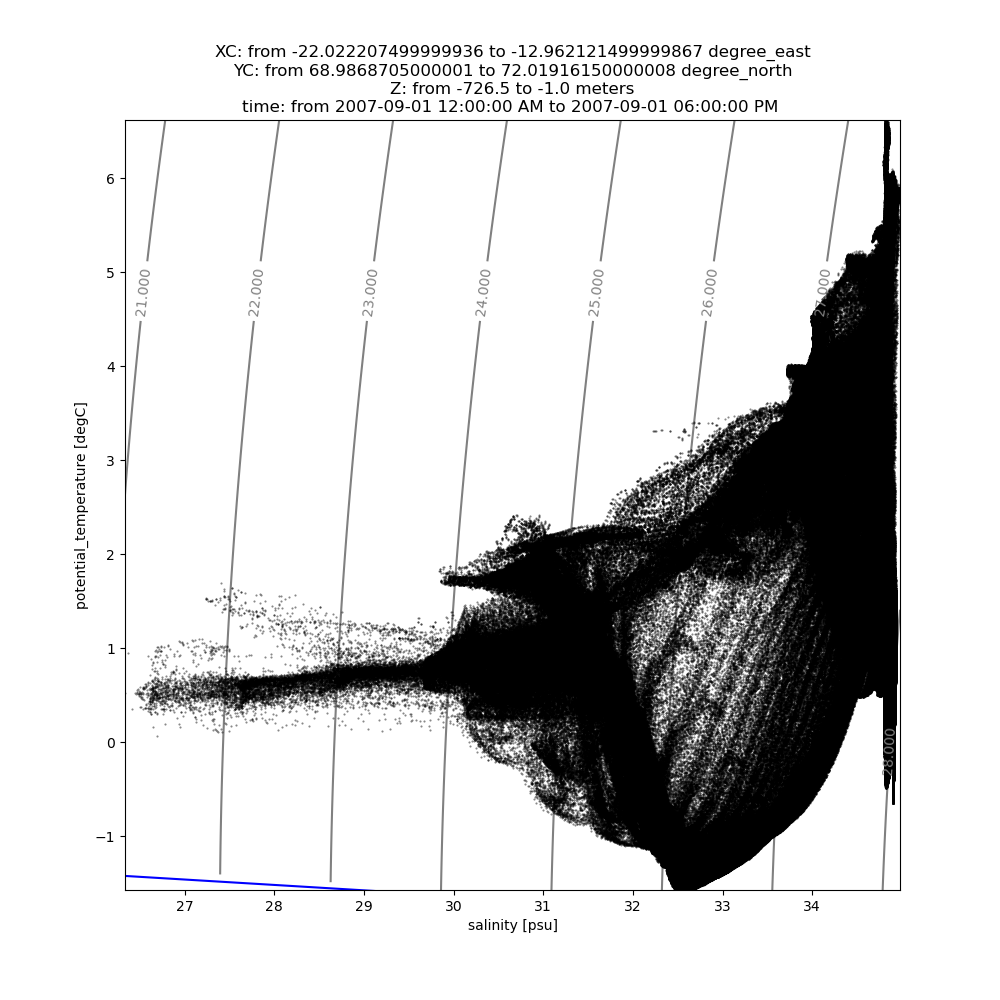
\includegraphics[width=1\textwidth]{TempvsSalinity}
\caption{Temperature vs Salinity plot using TS\_diagram() method}
\label{fig:TempvsSalinity}
\end{figure}

\begin{figure}
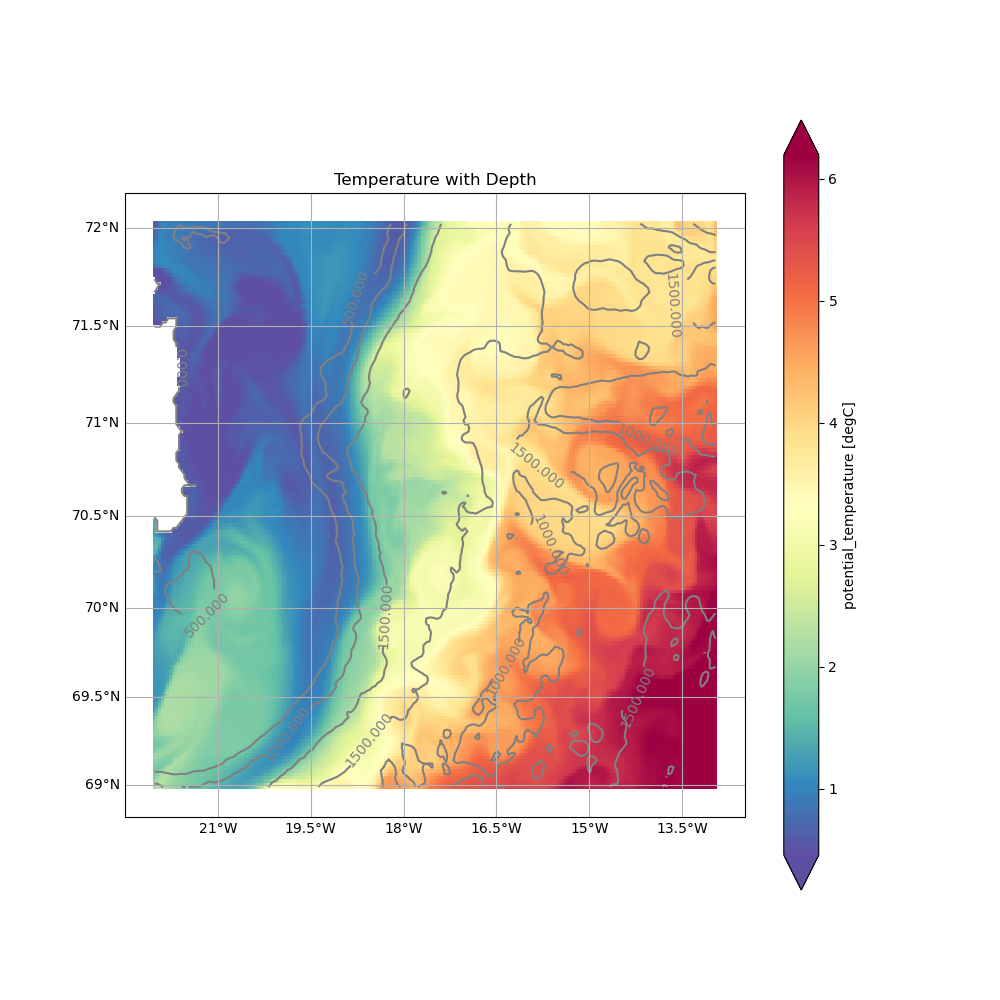
\includegraphics[width=1\textwidth]{TempwithDepth}
\caption{Temperature with Depth plotted as Contour channel using horizontal\_section() method}
\label{fig:TempwithDepth}
\end{figure}

Both of the plot were generated successfully. It can be seen that on figure \ref{fig:TempvsSalinity}, along with the plot some data like XC and YC is also being displayed. I don't actually get the significance of it. Also from the plot, it can be observed that salinity increases in a slow manner with the increment of temperature. 

On figure \ref{fig:TempwithDepth} the horizontal\_section() function creates a plot of temperature and shows a colorbar with the plot that shows the color for different temperature. In this plot we can also see the depth through the contour of the plot.Horizontal axis of this plot indicates the longitude and vertical axis indicates the latitude. 












\section{Conclusions}
I have explored two plotting feature that is provided by OceanSpy python module and found out that this package generates useful plots for ocean scientists and professionals. I could not interpret much of the use cases of the module due to lack of domain knowledge regarding ocean data. I intend to explore the module in a later time with a better understanding of ocean data and related knowledge about oceanographic visualizations and ocean current simulation models.

\end{document}